\section{Person Isolation}
\label{testing:person isolation}
This section details the testing of the depth based person isolation.\\

\subsection{Isolating Multiple Subjects}
During the design of depth based person isolation in Section \ref{imp:depth based isolation}, the isolation was determined to be sufficient for one person. Further testing was conducted on multiple subjects to confirm that the method would work on many people, rather than only the subject in Figure \ref{fig:depth and hand based cut off}. Figure \ref{fig:multiple subjects isolated} show the behaviour of the isolation method on the aforementioned multiple subjects. From this figure, the isolation method can be said to work consistently on many subjects.\\

\begin{figure}[h]
\begin{center}
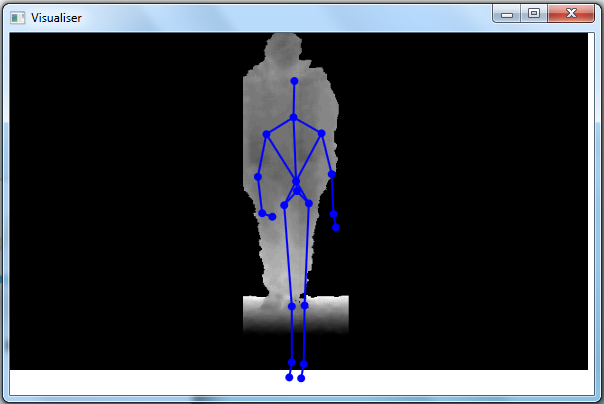
\includegraphics[scale=0.3]{images/bernie_iso} 
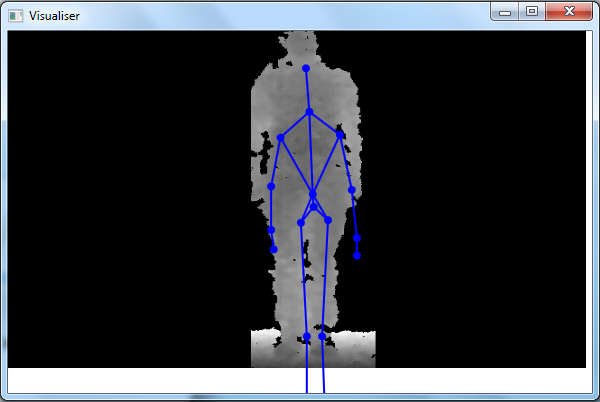
\includegraphics[scale=0.3]{images/page} 
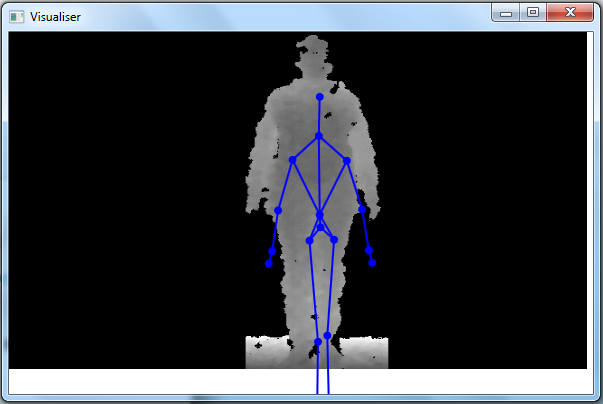
\includegraphics[scale=0.3]{images/steffat} 
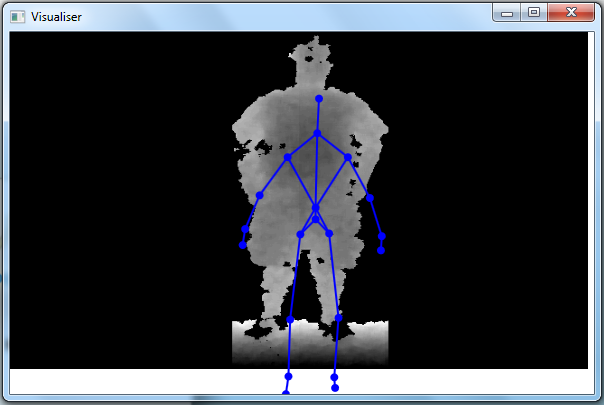
\includegraphics[scale=0.3]{images/wilkoiso} 
\end{center}
\caption{Multiple subjects isolated.}
\label{fig:multiple subjects isolated}
\end{figure} 

\subsection{Floor Removal}
As previous noted in Sections \ref{design:depth based isolation} and \ref{imp:depth based isolation}, the depth based cut off leaves the floor underneath the person as an unwanted artifact in the final point cloud. Fortunately, the floor can be removed at the point cloud level as suspected. An example of this action is shown in Figure \ref{fig:floor removal}.\\

\begin{figure}[h]
\begin{center}
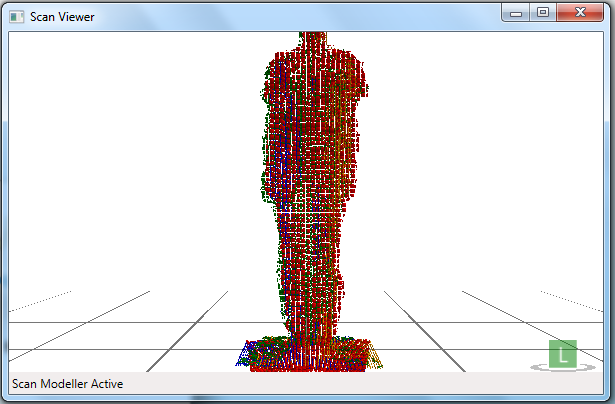
\includegraphics[scale=0.3]{images/greg_feet}
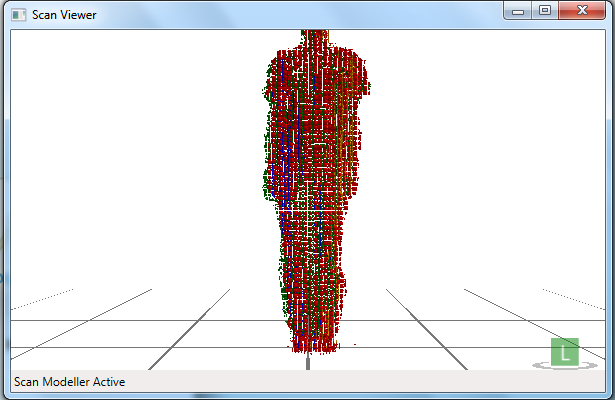
\includegraphics[scale=0.3]{images/greg_nofeet} 
\end{center}
\caption{Left: The point cloud with the floor. Right: After floor removal.}
\label{fig:floor removal}
\end{figure} 